\documentclass[12pt]{article}
\usepackage{blindtext}
\usepackage{graphicx}
\usepackage[margin=0.6in]{geometry}
\title{Deep Learning for Spech-Rap-Singing Audio Classification}
\date{\today}
\author{Axel Ind, Msc. Computer Science}
\begin{document}
\maketitle

\section*{Abstract}
I have implemented two different deep learning architecture to learn the 3-output classification of 3 second music clips with a $16kHz$ sample rate. Implementations make use of Librosa for audio-preprocessing, and the Keras environment for model implementation. Labels are learned with a 13-variable MFCC as input data. Results achieved are: 98\%, 89\% accuracy on test data for the CNN and MLP respectively.

\section{Audio-Preprocessing}
\begin{enumerate}
\item Confirmed that each sample match the three second length and $16kHz$ sample rate.
\item Used \texttt{Librosa} to extract signal data from each sample.
\item Used \texttt{Librosa} to convert signal data to 13-variable MFCC.
\item Stored data in a \texttt{.json} file with format: (`label':\{...\},`MFCC':\{[...]\}).
\end{enumerate}
\section{Architectures}
\subsection{Classic Dense Network}
\begin{itemize}
\item Layer 1: Flatten Layer (to reduce MFCC to vector)
\item Layer 2-4: Dense Layers (relu, dropout) with 512, 256, and 64 nodes, respectively. 
\item Layer 5: Output Layer (3 nodes, softmax)
\end{itemize}
\subsection{Convolutional Neural Network}
\begin{itemize}
\item Layers 1-6 alternate this standard pair of convolution-oriented layers giving a total of three Convolutional Layers:
\begin{itemize}
\item a: 2DConvolution (32 filters, $3\times 3$ kernel size, relu)
\item b: MaxPool (pool\_size=$3\times 3$, strides=$2\times 2$, relu)  with Batch Normalisation.
\end{itemize}
\item Layer 3: Dense Layer (relu, dropout) with 64 nodes.
\item Layer 4: Output Layer (3 nodes, softmax)

\end{itemize}
\section{Results}
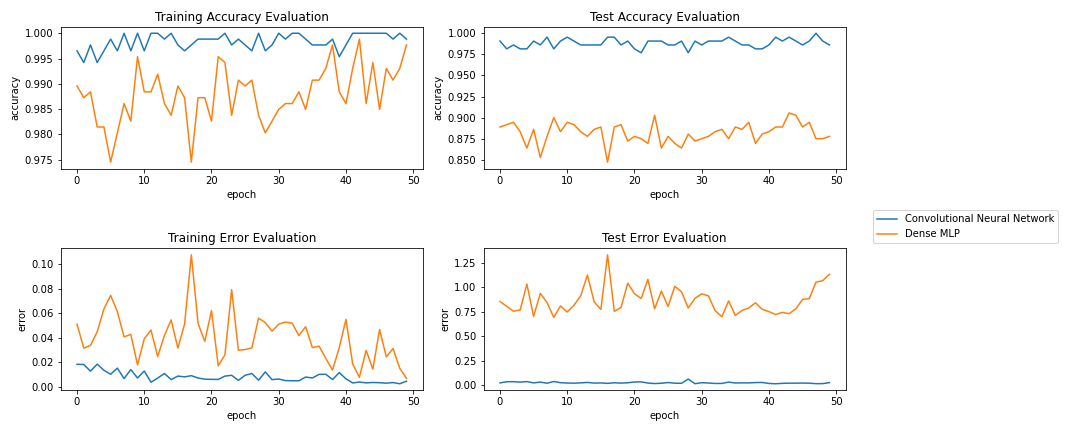
\includegraphics[width= \textwidth]{accuracyMeasures.png}
\subsection{CNN Results}
With $\mu=0.0001, \bar{t}=5.42s$
\begin{itemize}
\item \textbf{Average Accuracy}: 94.657\%
\item \textbf{Max Accuracy}: 99\%
\end{itemize}

\subsection{Dense Network Results}
With $\mu=0.0001, \textit{dropout}=0.1, \bar{t}=4.58s$
\begin{itemize}
\item \textbf{Average Accuracy}: 89.657\%
\item \textbf{Max Accuracy}: 95.735\%
\end{itemize}



\section{Limitations}
\begin{itemize}
\item Training can currently include different features from the same person's voice as the test set.
\item The amount of training data currently available is rather limited. Perturbating the existing data could potentially increase accuracy.
\item Hyper-parameter optimisation will be necessary.
\item An LSTM solution was implemented but does not run in \texttt{Python 3.8} and I am still troubleshooting compatibility.

\end{itemize}













\end{document}